%%%%%%%%%%%%%%%%%%%%%%%%%%%%%%%%%%%%%%%%%
% University/School Laboratory Report
% LaTeX Template
% Version 3.1 (25/3/14)
%
% This template has been downloaded from:
% http://www.LaTeXTemplates.com
%
% Original author:
% Linux and Unix Users Group at Virginia Tech Wiki 
% (https://vtluug.org/wiki/Example_LaTeX_chem_lab_report)
%
% License:
% CC BY-NC-SA 3.0 (http://creativecommons.org/licenses/by-nc-sa/3.0/)
%
%%%%%%%%%%%%%%%%%%%%%%%%%%%%%%%%%%%%%%%%%

%----------------------------------------------------------------------------------------
%	PACKAGES AND DOCUMENT CONFIGURATIONS
%----------------------------------------------------------------------------------------

% please be aware to install sudo apt-get install texlive-science

\documentclass{article}

%\usepackage[version=3]{mhchem} % Package for chemical equation typesetting
\usepackage{siunitx} % Provides the \SI{}{} and \si{} command for typesetting SI units
\usepackage{graphicx} % Required for the inclusion of images
\usepackage{natbib} % Required to change bibliography style to APA
\usepackage{amsmath} % Required for some math elements 
\usepackage{fullpage}
\usepackage{todonotes} %todonoes
\usepackage{listings}
\setlength\parindent{0pt} % Removes all indentation from paragraphs

\renewcommand{\labelenumi}{\alph{enumi}.} % Make numbering in the enumerate environment by letter rather than number (e.g. section 6)

%\usepackage{times} % Uncomment to use the Times New Roman font

%----------------------------------------------------------------------------------------
%	DOCUMENT INFORMATION
%----------------------------------------------------------------------------------------

\title{JEngine Documentation} % Title

\author{BP2014W1 Team} % Author name

\date{\today} % Date for the report

\begin{document}

\maketitle % Insert the title, author and date


\begin{center}
\begin{tabular}{l r}
Date Performed: & January 1, 2015 \\ % Date the experiment was performed
%Betreuer: & Andreas Meyer \\ % Partner names
%& Marcin Hewelt \\
%Instructor: & Professor Dr Mathias Weske % Instructor/supervisor
\end{tabular}
\end{center}

\listoftodos %displaying open todos

%----------------------------------------------------------------------------------------
%	SECTION 0 
%----------------------------------------------------------------------------------------

% If you wish to include an abstract, uncomment the lines below
\begin{abstract}
This documentation is created in the context of the bachelor project BP2014W1 at the research group of Prof. Dr. Mathias Weske. The goal of the project was to implement an Engine for supporting the concept of \textit{Production Case Management} (PCM) in order to provide a proof of concept and a prototype for several uses cases of Bosch Sofware Innovations. This document serves as a detailed documentation of the result.   
\end{abstract}

%\tableofcontents
%\listoffigures
%\listoftables
%\lstlistoflistings
%\listofsymbols{ll}{$w$ & The weight vector}
%\acknowledgements{Thanks to no one.}
%\dedicatory{To \dots}
%\mainmatter

%----------------------------------------------------------------------------------------
%	SECTION 1
%----------------------------------------------------------------------------------------


%
%
\section{Introduction}
Production Case Management describes a flexible alternative to traditional processmanagement which focuses the modelling and execution of static, predefined processes. PCM, on the contrary, supports the usage of processvariants granting simplification of complex processmodels and flexibility in the execution by splitting complex processes into less complex fragments.

%
%
\section{JEngine}
Overall JEngine

\begin{figure}
\centering
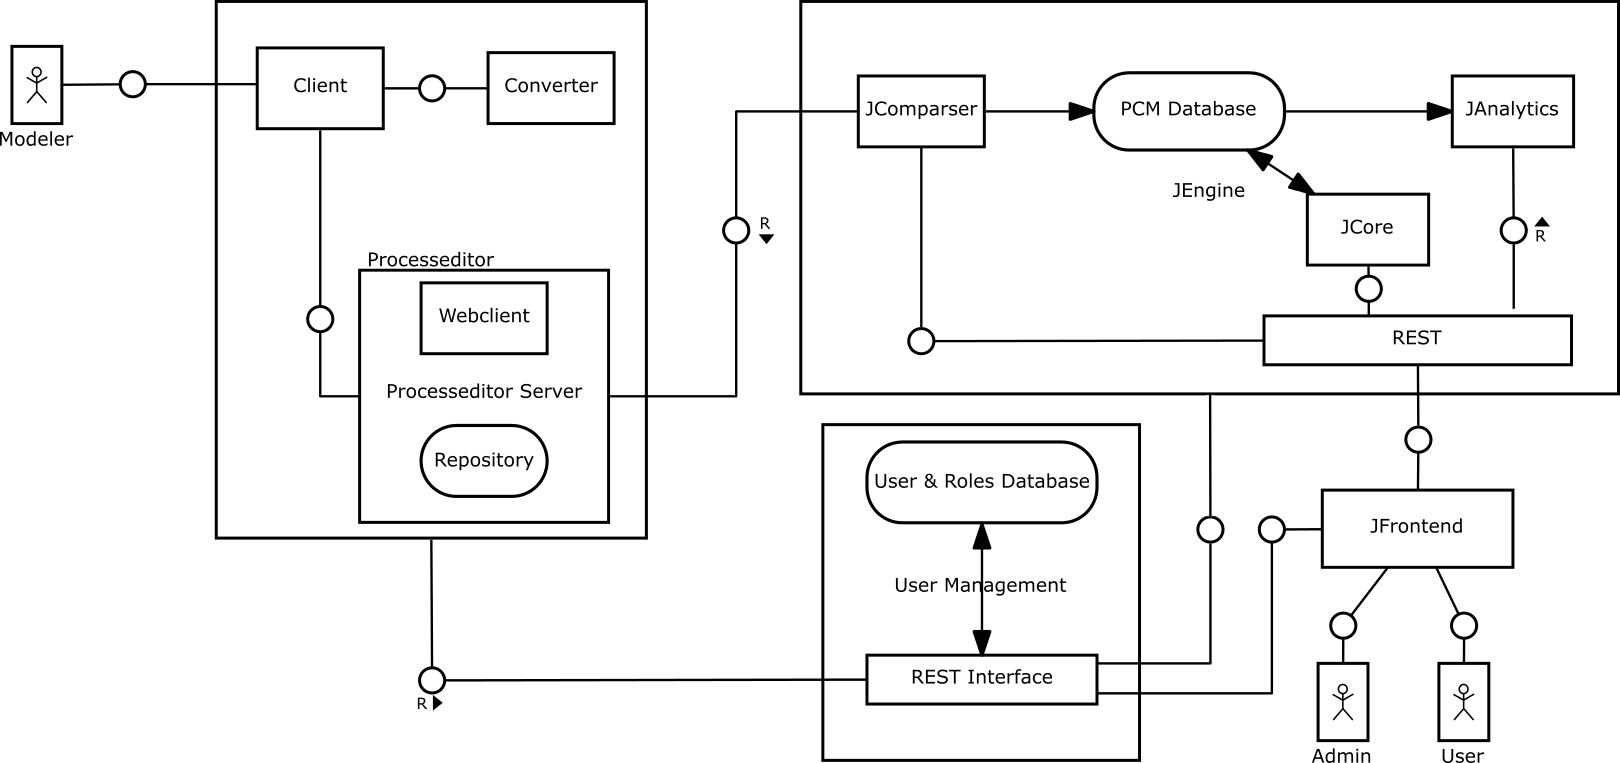
\includegraphics[width=6in]{img/fmc-architecture-v2_4.png}
\caption{Meta Modell von PCM.}
\label{fig:PCMmetaModell}
\end{figure}

%%%%%%%%%%%%%%%%%%%%%%%%%% JCore %%%%%%%%%%%%%%%%%%%%%%%%%% 

% Consider using 
%
%
\subsection{JCore}
The JCore contains several main components of our engine. Those contain the evaluation of the database and the enablement of activities in the ExecutionService etc.\\
In the JCore reside some of the most fundamental funtionalities that our engine offers. They include the possibility to run activities sequentially. Supported activity-types are user-task and email-task.\\
With PCM activities can be enabled from controllflow or dataflow point of view. That is the reason why we support dataobjects and their state transitions. Further activities can be referenced in PCM, which has the effect during execution, that referenced activities, which are enabled and share the same set of pre- and postconditions, can both switch to the state 'running' if one of them is being activated.\\
Also PCM-fragments consist of a subset of BPMN. Currently we support start- and end-events, activities and XOR- and AND-Gateways.


\subsubsection{Class diagram}

The ExecutionService is the class that manages the complete JCore. The ExecutionService manages all ScenarioInstances and provides methods to interact with a scenario instance, for example to do an activity.\\
The ScenarioInstance represents an instance of a PCM scenario. It saves all FragmentInstances, ControlNodeInstances and DataObjectInstances. If a ScenarioInstance get initialized it initializes all FragmentInstances and DataObjectInstances.\\
The DataObjectInstances represent PCM data objects. They have a state and list of all there DataAttributeInstances. The DataAttributeInstance represent the data attributes and save the value and the type of the attribute.\\
The FragmentInstances have one function they initialize all ControlNodeInstances.
ControlNodeInstances are ActivityInstances and GatewayInstances which are shown in the PCM model. All ControlNodeInstances have a StateMachine,  a IncomingBehavior and a OutgoingBehavior. The StateMachine controls the state of the ControlNodeInstance and does the state transitions. The IncomingBehavior controls the incoming control flow. This is important for PCM gateways, because this behavior decides if a AND gateway for example can be activated. The OutgoingBehavior controls the outgoing control flow. For Example the data object output states for an activity are set here.\\
An ActivityInstance also have an TaskExecutionBehavior this behavior manages all things that happens if you execute the activity. This can be the HumanTaskExecutionBehavior that sets the data attribute states or a service task execution behavior like the EmailTaskExecutionBehavior that send automatic an eMail.\\

\begin{figure}[h!]
\centering
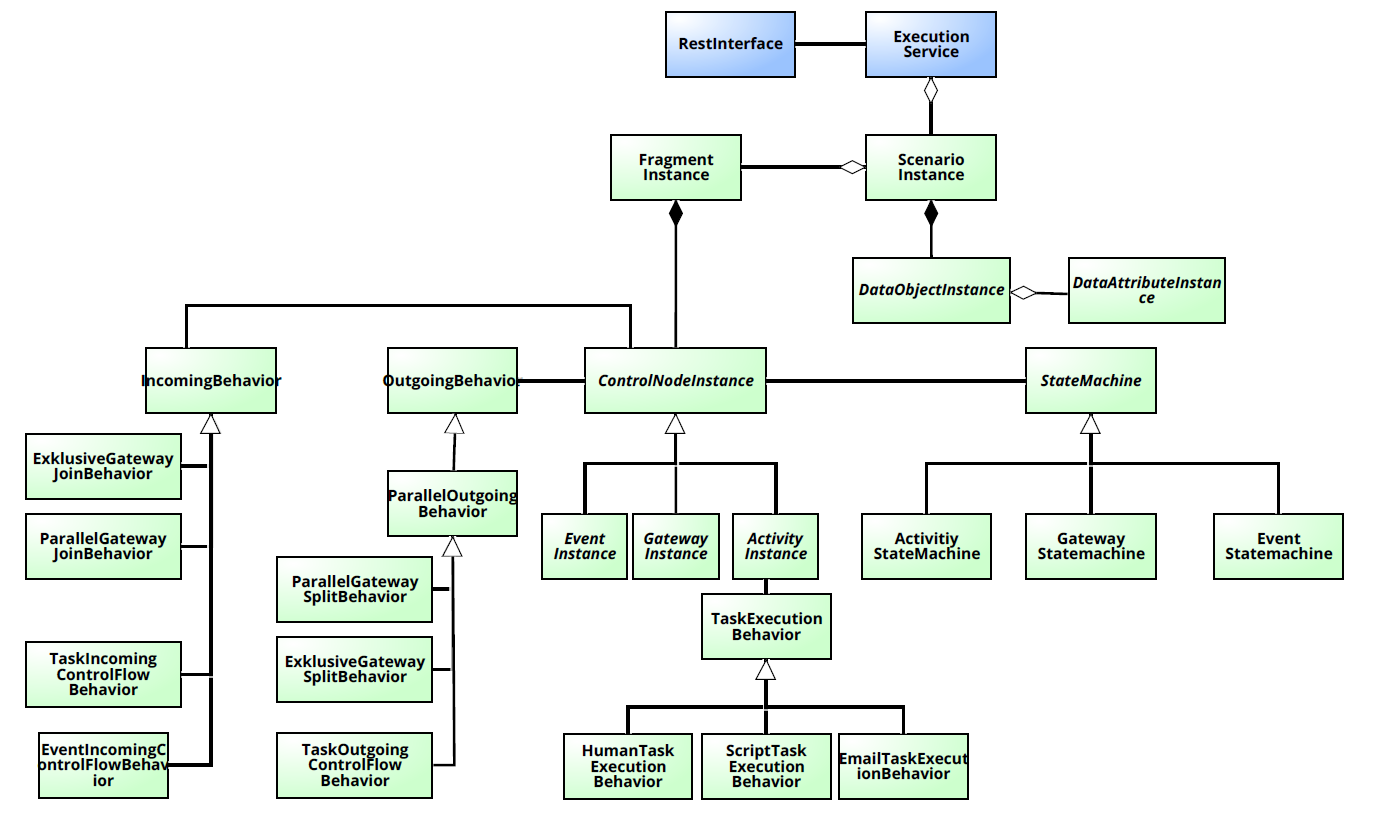
\includegraphics[width=6in]{img/ClassDiagramm.png}
\caption{userview}
\label{fig:userview}
\end{figure}

\subsubsection{E-Mail-Tasks}
\label{jCore:MailTask}
The JEngine supports the execution of E-MailTasks. All of the E-Mail configurations are saved in the database in table \textit{emailconfiguration}. Every E-Mail-Task which is modeled as described in section \ref{pe:email} gets its own database entry whith the corresponding controlnodeID (that's the databaseID, not the modelID from the XML) of the Mail Task.\\
The default template holds the databaseID -1. The values of the attributes from the default template are copied for each individual E-Mail-Task. In so far, the receivermailaddress, sendmailaddress, subject and messagecontent from the default template are used, if not specified differently. The databaseID and the controlnodeID are set automatically. If you wish to make an own configuration for the Mail Task, you can use the frontEnd 
\begin{math}(Admin\rightarrow Mail Config)\end{math}
by selecting the scenario, choosing the Activity and clicking on \textit{Show Details}. After a window with the default content opens, you can enter the receiver, subject, and message. Otherwise you can also change the values in the database.\\
\textbf{Attributes.} It is possible to access the values of dataAttributes in the message content, subject or e-Mail address by typing the following expression:
\begin{align}
\textbf{\#dataobjectName.dataobjectAttributeName} \nonumber
\end{align}
This expression gets replaced by the value of \textit{dataobjectAttributeName} which is an attribute of \textit{dataobjectName}.

\subsubsection{WebServiceTasks}
The JEngine supports the execution of WebServiceTasks. All of the WebService configurations are saved in the database in tables \textit{webservicetasklink, webservicetaskpost, webservicetaskattribute}. Initial Webservice Tasks have no configuration entries in the database. The user have to configure the Tasks.\\
In the database table \textit{webservicelink} is the method of the request defined. This can be \textit{GET, PUT or POST}.\\
In the database table \textit{webservicepost} gets the JSON for the PUT/POST request saved. The information from the dataobject and dataattributes can be used in the request. To access the values and states you have to type following expression:
\textbf{\#dataobjectName.dataobjectAttributeName} \nonumber for the attribute value or
\textbf{\#dataobjectName} \nonumber for the dataobject state.\\
In the database table \textit{webserviceattribute} is defined which values from the JSON are saved in which dataattribute. The Engine uses the \textit{key} to know how to access the JSON. The \textit{order} ist the order in which the \textit{keys} are used.
%
%

\subsubsection{XOR Gateways}

The JCore can execute XOR Gateways. The syntax of the conditions is shown by the following grammar. Expressions like \textit{#Dataobject.Dataattribute} or \textit{#Dataobject} are replaced with Dataattribute values and Dataobject states.\\
\begin{lstlisting}

expression  ::=     expr2 (OPERATOR expr2)*;
expr2       ::=     NAME COMPARISON NAME;
NAME        ::=     CHARAC | CHARAC  DOT CHARAC;
CHARAC      ::=     [#]('A'..'Z' | 'a'..'z' | '0'..'9')+;
COMPARISON  ::=     '=' | '<' | '>' | '<=' | '>=';
DOT         ::=     '.';
OPERATOR    ::=     ' & ' | ' | ' | '&' | '|';

\end{lstlisting}

\subsubsection{REST-API}

veraltet

\iffalse
Um eine Kommunikation zwischen unseren verschieden Elementen der Engine und des Front-Ends zu ermöglichen, haben wir uns für ein REST-Interface entschieden. Dabei unterstützen wir bisher 2 Methoden: GET und POST.
\begin{enumerate}
%hier beginnt Aufzählung unserer REST Methoden
\item \textbf{@GET:}\\
Die GET-Requests existieren, um den Nutzern der Engine über ein User Interface eine Möglichkeit zu bieten, einzusehen welche Aktivitäten noch zu bearbeiten sind (also offen sind) bzw. welche Aktivitäten zu welcher Scenarioinstanz gehören und ähnliches. \\

1.1.\\ Um offene bzw. geschlossene Aktivitäten einer ScenarioInstanz ausgegeben zu bekommen, muss ein GET mit folgender URL ausgeführt werden:\\
\textbf{\textit{http://172.16.64.113:8080/JEngine/Scenario/\\\{ScenarioID\}/\{ScenarioInstanceID\}/\{Status\}}}\\

\textbf{Variablen die benutzt werden:}\\
\textit{ScenarioID:} hier wird die ID des Scenarios erwartet. Dabei handelt es sich um einen Integer-Wert.\\
\textit{ScenarioInstanceID:} hier wird die ID der ScenarioInstanz erwartet. Dabei handelt es sich um einen Integer-Wert.\\
\textit{Status:} Der Status ist vom Typ String und muss ein Element der Menge\textbf{\textit{\{terminated, enabled\}}} sein.\\

\textbf{Dabei können folgende Fehler geworfen werden:}\\
\textit{Error: not a correct scenario instance}\\ Dies bedeutet das eine ScenarioInstanzID angegeben worden ist, die nicht existiert.\\
\textit{Error: status not clear}\\ Dieser Fehler besagt, dass ein Status angegeben wurde, der nicht der Menge \textbf{\textit{\{terminated, enabled\}}} entspricht.\\

1.2. \\Wenn man wissen möchte, welche Szenarien man in der JEngine starten kann, erhält man diese über folgende GET URL:\\
\textbf{\textit{http://172.16.64.113:8080/JEngine/Scenario/\\Show}}\\

1.3.\\ Um alle ScenarioInstanzen eines Szenarios zu bekommen, muss ein GET-Request mit folgender URL ausgeführt werden:\\
\textbf{\textit{http://172.16.64.113:8080/JEngine/Scenario/\\Instances/\{ScenarioID\}}}\\

\textbf{Variable die benutzt wird:}\\
\textit{ScenarioID:} Dabei handelt es sich um einen Integer, der die ID des zu betrachtenden Szenarios angibt.\\

\textbf{Dabei kann folgender Fehler geworfen werden:}\\
\textit{Error: not a correct scenario}\\ Dieser tritt auf, wenn eine ID übergeben wurde, die nicht existiert.\\

1.4.\\ Wenn man alle Datenobjekte in ihren entsprechenden Zuständen anzeigen möchte, bezogen auf eine ScenarioInstanz, muss ein GET-Request mit folgender URL ausgfeührt werden:\\
\textbf{\textit{http://172.16.64.113:8080/JEngine/Scenario/\\DataObjects/\{ScenarioID\}/\{ScenarioInstanceID\}}}\\

\textbf{Variablen die benutzt werden:}\\
\textit{ScenarioID:} hier wird die ID des Scenarios erwartet. Dabei handelt es sich um einen Integer-Wert.\\
\textit{ScenarioInstanceID:} hier wird die ID der ScenarioInstanz erwartet. Dabei handelt es sich um einen Integer-Wert.\\

\textbf{Dabei kann folgender Fehler geworfen werden:}\\
\textit{Error: not a correct scenario instance}\\ Wenn eine falsche ScenarioInstanzID angegeben wird, produziert es diesen Fehler.\\

1.5.\\ Um von einer SzenrioInstanzID die dazugehörige ScenrioID zu erhalten, kann ein GET-Request mit folgender URL ausgeführt werden:\\ 
\textbf{\textit{http://172.16.64.113:8080/JEngine/Scenario/\\Get/ScenarioID/\{ScenarioInstanceID\}}}\\

\textbf{Variable die benutzt wird:}\\
\textit{ScenarioInstanceID:} hier wird die ID der ScenarioInstanz erwartet. Dabei handelt es sich um einen Integer-Wert.\\

\textbf{Dabei kann folgender Fehler geworfen werden:}\\
\textit{Error: not a correct scenario instance} \\ Wurde eine ScenarioInstanzID angegeben, die nicht existiert, wird dieser Fehler geworfen.\\

1.6.\\ Wenn man eine AktivitätsInstanzId besitzt, und das dazugehörige Label wissen möchte, kann man einen GET-Request mit folgender URL ausführen:\\
\textit{\textbf{http://172.16.64.113:8080/JEngine/Scenario/\\ActivityID/\{Activity\}}}

\textbf{Variable die benutzt wird:}\\
\textit{Activity:} hier wird die ID der AktivitätsInstanz erwartet. Dabei handelt es sich um einen Integer-Wert.\\

\textbf{Dabei kann folgender Fehler geworfen werden:}\\
\textit{Error: not correct Activity ID}\\ Wurde eine AktivitätsInstanzID angegeben, die nicht existiert, wird dieser Fehler geworfen.\\

\item \textbf{@POST:}\\
Über POST-Request ist es möglich, Aktivitäten zu starten sowie gestartete Aktivitäten zu terminieren. Außerdem besteht auch die Möglichkeit ganze Szenarien zu starten, falls dies benötigt wird. All dies soll mit der Funktion ausgestattet sein, dass man dazu noch einen Kommentar abgeben kann.\\

2.1.\\ Um über einen POST-Request Aktivitäten zu starten bzw. zu beenden, wird die folgende URL genutzt:\\
\textit{\textbf{http://172.16.64.113:8080/JEngine/Scenario/\\\{ScenarioID\}/\{ScenarioInstanceID\}/\\\{ActivityID\}/\{Status\}/comment}}\\

\textbf{Variablen die benutzt werden:}\\
\textit{ScenarioID:} hier wird die ID des Scenarios erwartet. Dabei handelt es sich um einen Integer-Wert.\\
\textit{ScenarioInstanceID:} hier wird die ID der ScenarioInstanz erwartet. Dabei handelt es sich um einen Integer-Wert.\\
\textit{ActivityID:} hier wird die ID der AktivitätsInstanz erwartet. Dabei handelt es sich um einen Integer-Wert.\\
\textit{Status:} Der Status ist vom Typ String und muss ein Element der Menge\textbf{\textit{\{terminate, begin\}}} sein.\\

\textbf{Im Fehlerfall:}\\
Wird versucht eine Aktivität zu starten, die nicht existiert bzw. eine Aktivität zu beenden, die gar nicht gestartet war, wird einem ein Boolean mit dem Wert \textit{false} zurückgegeben.\\

2.2.\\ Wenn eine neue Instanz eines Szenarios gestartet werden soll, nutzt man den POST-Request mit folgender URL:\\
\textit{\textbf{http://172.16.64.113:8080/JEngine/Scenario/\\Start/\{ScenarioID\}}}\\

\textbf{Variable die benutzt wird:}\\
\textit{ScenarioID:} hier wird die ID des Scenarios erwartet. Dabei handelt es sich um einen Integer-Wert.\\

\textbf{Im Fehlerfall:}\\
Wird versucht ein Szenario zu starten, das nicht existiert, wird einem ein Integer mit dem Wert \textit{-1} zurückgegeben.\\

\end{enumerate}


Default URL:
http://172.16.64.113:8080/JEngine/interface/\{version\}/\{language\}/?

as parameter:
scenario
returns all scenarios
 
scenario=1
returns all instances

scenario=1\& runtime
returns all instances with runtime

instanceid=1\& status=enabled
returns all enabled activities

activityid=2
returns all information for this activity

users
returns all users

roles
roles returns all roles


timestamp ISO-8601
\fi

for more informations about the REST please have a look at the REST Specification:
https://github.com/BP2014W1/JEngine/blob/dev/docu/JEngine_REST_Specs.pdf


%
%
\subsubsection{ExecutionService}
The ExecutionService is the component that is being used by the REST-API. So this component of the JEngine is essential to process queries that have been received via the REST interface. It establishes a database-connection to run queries on it. Most queries require the ID of an object to gather more information. Additionaly there are methods to instantiate activities and whole scenarios respectively. instead

%
%
\subsection{JCore}
The JCore contains several main components of our engine. Those contain the evaluation of the database and the enablement of activities in the ExecutionService etc.\\
In the JCore reside some of the most fundamental funtionalities that our engine offers. They include the possibility to run activities sequentially. Supported activity-types are user-task and email-task.\\
With PCM activities can be enabled from controllflow or dataflow point of view. That is the reason why we support dataobjects and their state transitions. Further activities can be referenced in PCM, which has the effect during execution, that referenced activities, which are enabled and share the same set of pre- and postconditions, can both switch to the state 'running' if one of them is being activated.\\
Also PCM-fragments consist of a subset of BPMN. Currently we support start- and end-events, activities and XOR- and AND-Gateways.


\subsubsection{Class diagram}

The ExecutionService is the class that manages the complete JCore. The ExecutionService manages all ScenarioInstances and provides methods to interact with a scenario instance, for example to do an activity.\\
The ScenarioInstance represents an instance of a PCM scenario. It saves all FragmentInstances, ControlNodeInstances and DataObjectInstances. If a ScenarioInstance get initialized it initializes all FragmentInstances and DataObjectInstances.\\
The DataObjectInstances represent PCM data objects. They have a state and list of all there DataAttributeInstances. The DataAttributeInstance represent the data attributes and save the value and the type of the attribute.\\
The FragmentInstances have one function they initialize all ControlNodeInstances.
ControlNodeInstances are ActivityInstances and GatewayInstances which are shown in the PCM model. All ControlNodeInstances have a StateMachine,  a IncomingBehavior and a OutgoingBehavior. The StateMachine controls the state of the ControlNodeInstance and does the state transitions. The IncomingBehavior controls the incoming control flow. This is important for PCM gateways, because this behavior decides if a AND gateway for example can be activated. The OutgoingBehavior controls the outgoing control flow. For Example the data object output states for an activity are set here.\\
An ActivityInstance also have an TaskExecutionBehavior this behavior manages all things that happens if you execute the activity. This can be the HumanTaskExecutionBehavior that sets the data attribute states or a service task execution behavior like the EmailTaskExecutionBehavior that send automatic an eMail.\\

\begin{figure}[h!]
\centering
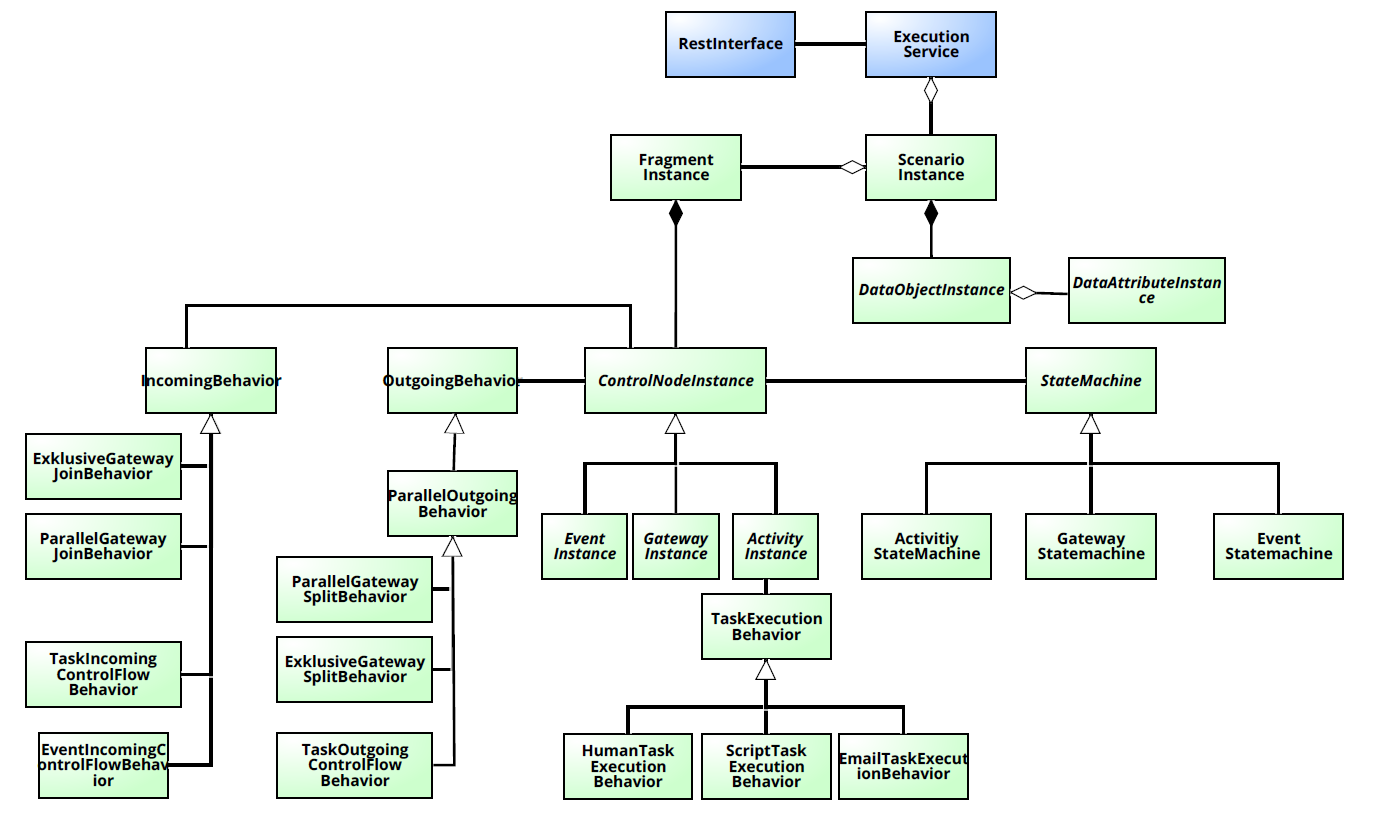
\includegraphics[width=6in]{img/ClassDiagramm.png}
\caption{userview}
\label{fig:userview}
\end{figure}

\subsubsection{E-Mail-Tasks}
\label{jCore:MailTask}
The JEngine supports the execution of E-MailTasks. All of the E-Mail configurations are saved in the database in table \textit{emailconfiguration}. Every E-Mail-Task which is modeled as described in section \ref{pe:email} gets its own database entry whith the corresponding controlnodeID (that's the databaseID, not the modelID from the XML) of the Mail Task.\\
The default template holds the databaseID -1. The values of the attributes from the default template are copied for each individual E-Mail-Task. In so far, the receivermailaddress, sendmailaddress, subject and messagecontent from the default template are used, if not specified differently. The databaseID and the controlnodeID are set automatically. If you wish to make an own configuration for the Mail Task, you can use the frontEnd 
\begin{math}(Admin\rightarrow Mail Config)\end{math}
by selecting the scenario, choosing the Activity and clicking on \textit{Show Details}. After a window with the default content opens, you can enter the receiver, subject, and message. Otherwise you can also change the values in the database.\\
\textbf{Attributes.} It is possible to access the values of dataAttributes in the message content, subject or e-Mail address by typing the following expression:
\begin{align}
\textbf{\#dataobjectName.dataobjectAttributeName} \nonumber
\end{align}
This expression gets replaced by the value of \textit{dataobjectAttributeName} which is an attribute of \textit{dataobjectName}.

\subsubsection{WebServiceTasks}
The JEngine supports the execution of WebServiceTasks. All of the WebService configurations are saved in the database in tables \textit{webservicetasklink, webservicetaskpost, webservicetaskattribute}. Initial Webservice Tasks have no configuration entries in the database. The user have to configure the Tasks.\\
In the database table \textit{webservicelink} is the method of the request defined. This can be \textit{GET, PUT or POST}.\\
In the database table \textit{webservicepost} gets the JSON for the PUT/POST request saved. The information from the dataobject and dataattributes can be used in the request. To access the values and states you have to type following expression:
\textbf{\#dataobjectName.dataobjectAttributeName} \nonumber for the attribute value or
\textbf{\#dataobjectName} \nonumber for the dataobject state.\\
In the database table \textit{webserviceattribute} is defined which values from the JSON are saved in which dataattribute. The Engine uses the \textit{key} to know how to access the JSON. The \textit{order} ist the order in which the \textit{keys} are used.
%
%

\subsubsection{XOR Gateways}

The JCore can execute XOR Gateways. The syntax of the conditions is shown by the following grammar. Expressions like \textit{#Dataobject.Dataattribute} or \textit{#Dataobject} are replaced with Dataattribute values and Dataobject states.\\
\begin{lstlisting}

expression  ::=     expr2 (OPERATOR expr2)*;
expr2       ::=     NAME COMPARISON NAME;
NAME        ::=     CHARAC | CHARAC  DOT CHARAC;
CHARAC      ::=     [#]('A'..'Z' | 'a'..'z' | '0'..'9')+;
COMPARISON  ::=     '=' | '<' | '>' | '<=' | '>=';
DOT         ::=     '.';
OPERATOR    ::=     ' & ' | ' | ' | '&' | '|';

\end{lstlisting}

\subsubsection{REST-API}

veraltet

\iffalse
Um eine Kommunikation zwischen unseren verschieden Elementen der Engine und des Front-Ends zu ermöglichen, haben wir uns für ein REST-Interface entschieden. Dabei unterstützen wir bisher 2 Methoden: GET und POST.
\begin{enumerate}
%hier beginnt Aufzählung unserer REST Methoden
\item \textbf{@GET:}\\
Die GET-Requests existieren, um den Nutzern der Engine über ein User Interface eine Möglichkeit zu bieten, einzusehen welche Aktivitäten noch zu bearbeiten sind (also offen sind) bzw. welche Aktivitäten zu welcher Scenarioinstanz gehören und ähnliches. \\

1.1.\\ Um offene bzw. geschlossene Aktivitäten einer ScenarioInstanz ausgegeben zu bekommen, muss ein GET mit folgender URL ausgeführt werden:\\
\textbf{\textit{http://172.16.64.113:8080/JEngine/Scenario/\\\{ScenarioID\}/\{ScenarioInstanceID\}/\{Status\}}}\\

\textbf{Variablen die benutzt werden:}\\
\textit{ScenarioID:} hier wird die ID des Scenarios erwartet. Dabei handelt es sich um einen Integer-Wert.\\
\textit{ScenarioInstanceID:} hier wird die ID der ScenarioInstanz erwartet. Dabei handelt es sich um einen Integer-Wert.\\
\textit{Status:} Der Status ist vom Typ String und muss ein Element der Menge\textbf{\textit{\{terminated, enabled\}}} sein.\\

\textbf{Dabei können folgende Fehler geworfen werden:}\\
\textit{Error: not a correct scenario instance}\\ Dies bedeutet das eine ScenarioInstanzID angegeben worden ist, die nicht existiert.\\
\textit{Error: status not clear}\\ Dieser Fehler besagt, dass ein Status angegeben wurde, der nicht der Menge \textbf{\textit{\{terminated, enabled\}}} entspricht.\\

1.2. \\Wenn man wissen möchte, welche Szenarien man in der JEngine starten kann, erhält man diese über folgende GET URL:\\
\textbf{\textit{http://172.16.64.113:8080/JEngine/Scenario/\\Show}}\\

1.3.\\ Um alle ScenarioInstanzen eines Szenarios zu bekommen, muss ein GET-Request mit folgender URL ausgeführt werden:\\
\textbf{\textit{http://172.16.64.113:8080/JEngine/Scenario/\\Instances/\{ScenarioID\}}}\\

\textbf{Variable die benutzt wird:}\\
\textit{ScenarioID:} Dabei handelt es sich um einen Integer, der die ID des zu betrachtenden Szenarios angibt.\\

\textbf{Dabei kann folgender Fehler geworfen werden:}\\
\textit{Error: not a correct scenario}\\ Dieser tritt auf, wenn eine ID übergeben wurde, die nicht existiert.\\

1.4.\\ Wenn man alle Datenobjekte in ihren entsprechenden Zuständen anzeigen möchte, bezogen auf eine ScenarioInstanz, muss ein GET-Request mit folgender URL ausgfeührt werden:\\
\textbf{\textit{http://172.16.64.113:8080/JEngine/Scenario/\\DataObjects/\{ScenarioID\}/\{ScenarioInstanceID\}}}\\

\textbf{Variablen die benutzt werden:}\\
\textit{ScenarioID:} hier wird die ID des Scenarios erwartet. Dabei handelt es sich um einen Integer-Wert.\\
\textit{ScenarioInstanceID:} hier wird die ID der ScenarioInstanz erwartet. Dabei handelt es sich um einen Integer-Wert.\\

\textbf{Dabei kann folgender Fehler geworfen werden:}\\
\textit{Error: not a correct scenario instance}\\ Wenn eine falsche ScenarioInstanzID angegeben wird, produziert es diesen Fehler.\\

1.5.\\ Um von einer SzenrioInstanzID die dazugehörige ScenrioID zu erhalten, kann ein GET-Request mit folgender URL ausgeführt werden:\\ 
\textbf{\textit{http://172.16.64.113:8080/JEngine/Scenario/\\Get/ScenarioID/\{ScenarioInstanceID\}}}\\

\textbf{Variable die benutzt wird:}\\
\textit{ScenarioInstanceID:} hier wird die ID der ScenarioInstanz erwartet. Dabei handelt es sich um einen Integer-Wert.\\

\textbf{Dabei kann folgender Fehler geworfen werden:}\\
\textit{Error: not a correct scenario instance} \\ Wurde eine ScenarioInstanzID angegeben, die nicht existiert, wird dieser Fehler geworfen.\\

1.6.\\ Wenn man eine AktivitätsInstanzId besitzt, und das dazugehörige Label wissen möchte, kann man einen GET-Request mit folgender URL ausführen:\\
\textit{\textbf{http://172.16.64.113:8080/JEngine/Scenario/\\ActivityID/\{Activity\}}}

\textbf{Variable die benutzt wird:}\\
\textit{Activity:} hier wird die ID der AktivitätsInstanz erwartet. Dabei handelt es sich um einen Integer-Wert.\\

\textbf{Dabei kann folgender Fehler geworfen werden:}\\
\textit{Error: not correct Activity ID}\\ Wurde eine AktivitätsInstanzID angegeben, die nicht existiert, wird dieser Fehler geworfen.\\

\item \textbf{@POST:}\\
Über POST-Request ist es möglich, Aktivitäten zu starten sowie gestartete Aktivitäten zu terminieren. Außerdem besteht auch die Möglichkeit ganze Szenarien zu starten, falls dies benötigt wird. All dies soll mit der Funktion ausgestattet sein, dass man dazu noch einen Kommentar abgeben kann.\\

2.1.\\ Um über einen POST-Request Aktivitäten zu starten bzw. zu beenden, wird die folgende URL genutzt:\\
\textit{\textbf{http://172.16.64.113:8080/JEngine/Scenario/\\\{ScenarioID\}/\{ScenarioInstanceID\}/\\\{ActivityID\}/\{Status\}/comment}}\\

\textbf{Variablen die benutzt werden:}\\
\textit{ScenarioID:} hier wird die ID des Scenarios erwartet. Dabei handelt es sich um einen Integer-Wert.\\
\textit{ScenarioInstanceID:} hier wird die ID der ScenarioInstanz erwartet. Dabei handelt es sich um einen Integer-Wert.\\
\textit{ActivityID:} hier wird die ID der AktivitätsInstanz erwartet. Dabei handelt es sich um einen Integer-Wert.\\
\textit{Status:} Der Status ist vom Typ String und muss ein Element der Menge\textbf{\textit{\{terminate, begin\}}} sein.\\

\textbf{Im Fehlerfall:}\\
Wird versucht eine Aktivität zu starten, die nicht existiert bzw. eine Aktivität zu beenden, die gar nicht gestartet war, wird einem ein Boolean mit dem Wert \textit{false} zurückgegeben.\\

2.2.\\ Wenn eine neue Instanz eines Szenarios gestartet werden soll, nutzt man den POST-Request mit folgender URL:\\
\textit{\textbf{http://172.16.64.113:8080/JEngine/Scenario/\\Start/\{ScenarioID\}}}\\

\textbf{Variable die benutzt wird:}\\
\textit{ScenarioID:} hier wird die ID des Scenarios erwartet. Dabei handelt es sich um einen Integer-Wert.\\

\textbf{Im Fehlerfall:}\\
Wird versucht ein Szenario zu starten, das nicht existiert, wird einem ein Integer mit dem Wert \textit{-1} zurückgegeben.\\

\end{enumerate}


Default URL:
http://172.16.64.113:8080/JEngine/interface/\{version\}/\{language\}/?

as parameter:
scenario
returns all scenarios
 
scenario=1
returns all instances

scenario=1\& runtime
returns all instances with runtime

instanceid=1\& status=enabled
returns all enabled activities

activityid=2
returns all information for this activity

users
returns all users

roles
roles returns all roles


timestamp ISO-8601
\fi

for more informations about the REST please have a look at the REST Specification:
https://github.com/BP2014W1/JEngine/blob/dev/docu/JEngine_REST_Specs.pdf


%
%
\subsubsection{ExecutionService}
The ExecutionService is the component that is being used by the REST-API. So this component of the JEngine is essential to process queries that have been received via the REST interface. It establishes a database-connection to run queries on it. Most queries require the ID of an object to gather more information. Additionaly there are methods to instantiate activities and whole scenarios respectively.
\newpage

%%%%%%%%%%%%%%%%%%%%%%%%%% jcomparser %%%%%%%%%%%%%%%%%%%%%%%%%% 
%%
%%
\subsection{JComparser}  %status = done   GET(2/2) POST(1/1) 
\label{subsec:Comparser}

	%
    %%
	\subsubsection{Scenarios}
	
	\textbf{Get all available scenarios for import}\\
			\begin{tabular}{lll}
				http & GET & \texttt{jcomparser/scenarios}
			\end{tabular}
		\begin{flushleft}
			\begin{lstlisting}
{
    "ids":
        {
            "800682779972007735":"Coffee process",
            "635432698":"Coffee process",
            "932221086":"Kaffeeprozess"
        }
}
			\end{lstlisting}
			\captionof{json}{Example output of get all available scenarios from jcomparser}
		\end{flushleft}

	 	\textbf{Get image of scenario}\\
			\begin{tabular}{lll}
				http & GET & \texttt{jcomparser/scenarios/932221086/image/}
			\end{tabular}
		\begin{flushleft}
			\begin{lstlisting}
                \missingfigure{example scenario image}
			\end{lstlisting}
			\captionof{json}{Example output of get activies log}
		\end{flushleft}


	 	\textbf{POST launch import of scenario}\\
			\begin{tabular}{lll}
				http & POST & \texttt{jcomparser/scenarios/932221086/}
			\end{tabular}

%\newpage

%%%%%%%%%%%%%%%%%%%%%%%%%% jfrontend %%%%%%%%%%%%%%%%%%%%%%%%%% 
%%
%
\subsection{JFrontEnd}

to be edited: \\
* AngularJS based\\
* using Bootstrap framework\\
* attaching to JEngine REST calls\\
* structured with regards to the input of Bosch Software Innovations\\

\missingfigure{add example Sceenshots of jFrontend}

\begin{figure}
\centering
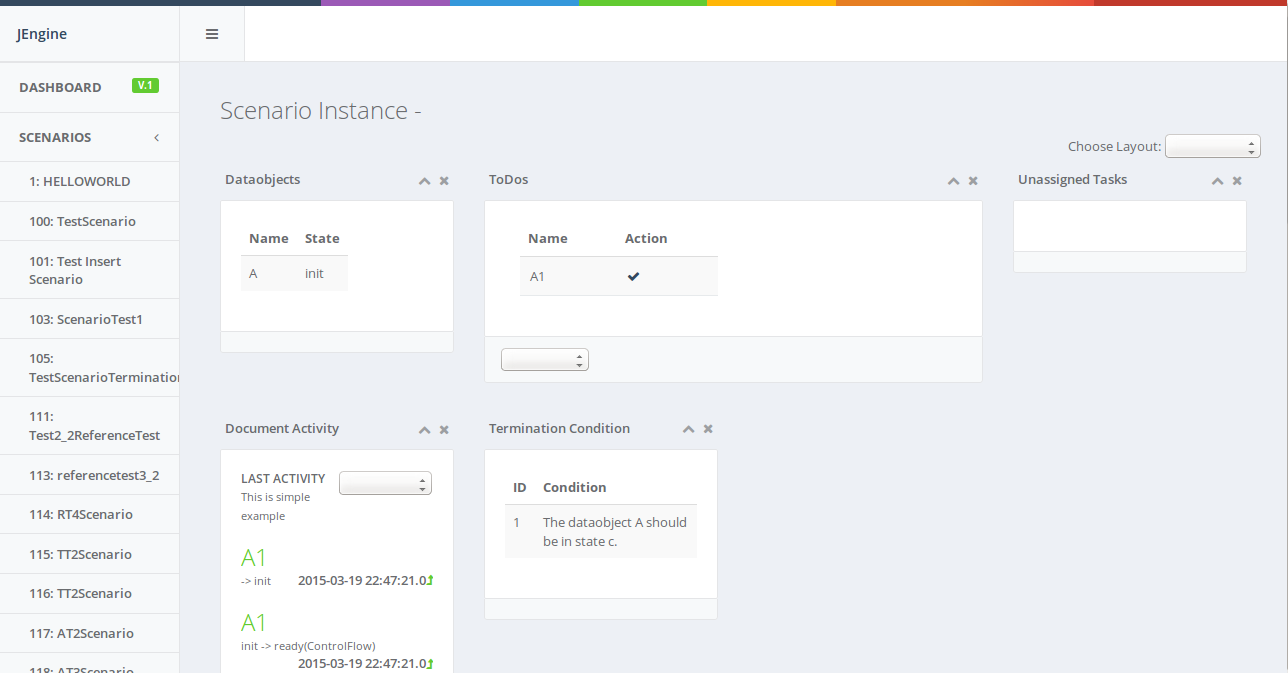
\includegraphics[width=3in]{img/userview.png}
\caption{userview}
\label{fig:userview}
\end{figure}

\begin{figure}
\centering
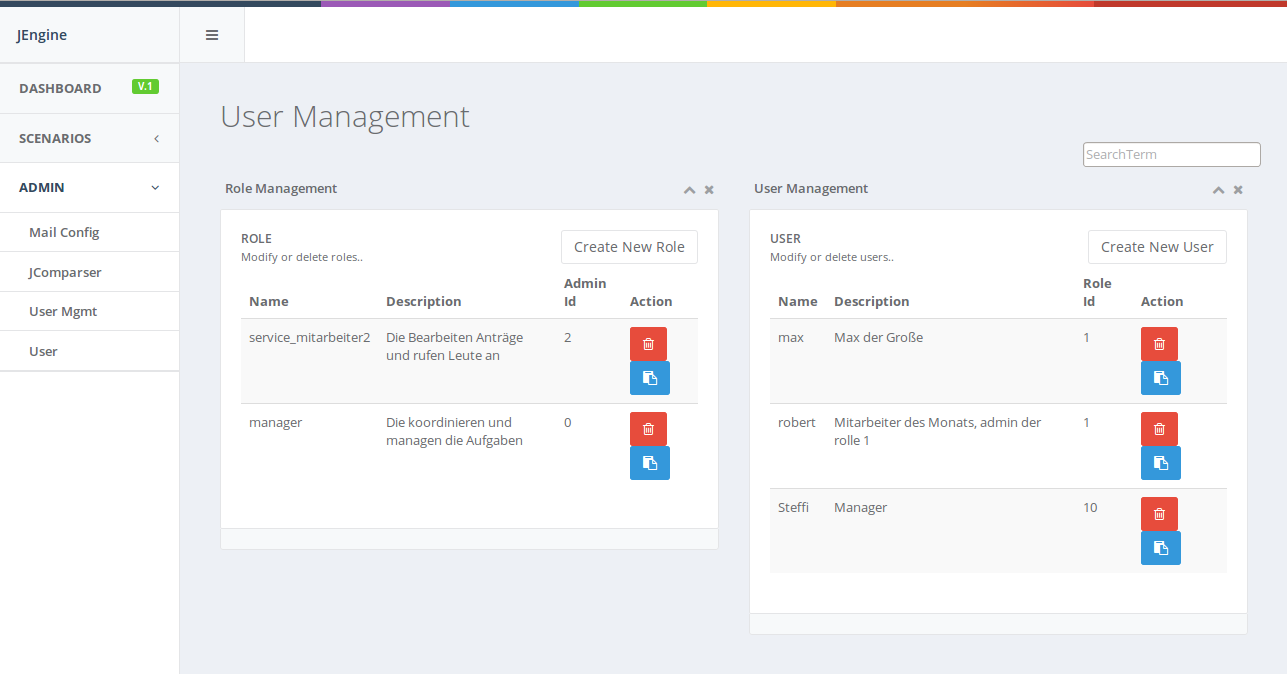
\includegraphics[width=3in]{img/user_management.png}
\caption{user management}
\label{fig:user_management}
\end{figure}

%\newpage

%%%%%%%%%%%%%%%%%%%%%%%%%% jdatabase %%%%%%%%%%%%%%%%%%%%%%%%%% 
%%
%
\subsection{JDatabase}

\missingfigure{database class diagram}
\\
The database is divided in three parts. Each part saves other specific information. There are the PCM Meta Model, PCM Model Instance and history. The PCM Meta Model part saves all PCM Scenarios.\\
The PCM Model Instance part saves all the information for the running and terminated instances.

\begin{figure}[h]
\centering
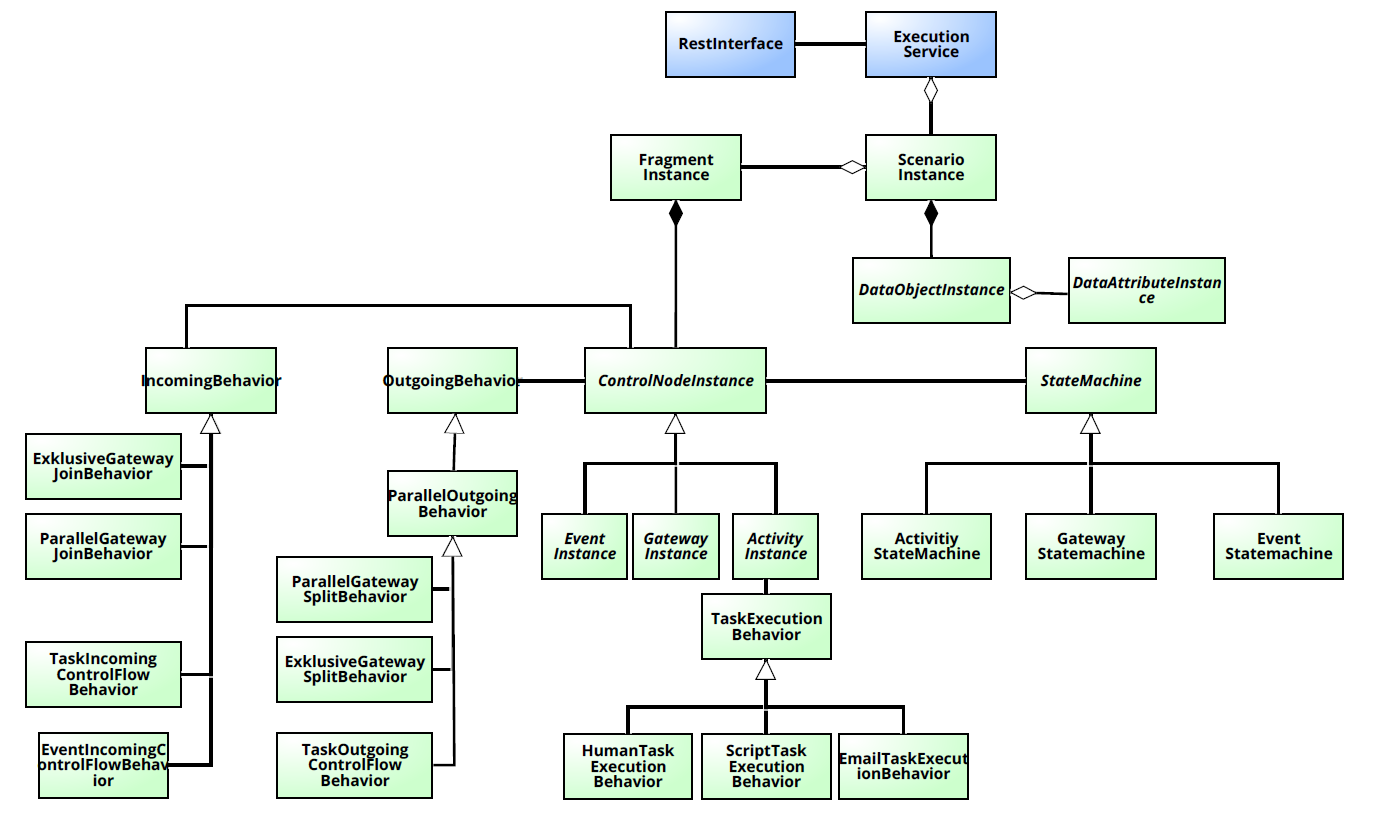
\includegraphics[width=6in]{img/ClassDiagramm.png}
\caption{userview}
\label{fig:userview}
\end{figure}
%\newpage


%%%%%%%%%%%%%%%%%%%%%%%%%% processeditor %%%%%%%%%%%%%%%%%%%%%%%%%% 

%
%
\section{Processeditor}

%
%
\section{PCM modelling using the Processeditor}
\label{pcm-modelling-using-the-processeditor}
This document explains how to use the Processeditor to create PCM models. A PCM-Process can be described by many PCM fragments and one PCM scenario.

%
%
\subsection{Preparations}
\label{preparations}
Currently you need both, the Processeditor Workbench and the Processeditor Server to model and Save PCM. You will use the Workbench for modelling and the Server as a global repository.

%
%
\subsection{PCM Fragments}
\label{pcm-fragments}
PCM Fragments are small Business Process models. They can be modelled using a subset of the BPMN-Notation:

\begin{itemize}
\itemsep1pt\parskip0pt\parsep0pt
\item
  Tasks
\item
  Events ** Blanko Start-Event ** Blanko End-Event
\item
  Gateways ** Parallel Gateway ** Exclusive Gateway
\item
  Data Objects
\item
  Sequence Flow
\item
  Data Flow
\end{itemize}

All these elements are offered by the model type PCM Fragment.

\subsubsection{E-Mail Tasks}
\label{pe:email}
The engine supports the execution of E-Mail Tasks. For the modelling you need to open the relevant fragment and add a normal (unspecified) task. In the properties-editor (you can open it with a right-click on the task and then choosing \textit{Properties...}) you simply set the stereotype to \textit{SEND}.\\
For configurating the E-Mail-Task and the execution in the engine, see section \ref{jCore:MailTask}.

%
%
\subsubsection{Marking a Task as Global}
\label{marking-a-task-as-global}
PCM allows to use the same task in more than one fragment. To do so

\begin{enumerate}
\def\labelenumi{\arabic{enumi}.}
\itemsep1pt\parskip0pt\parsep0pt
\item
  model the Task (in one scenario)
\item
  Save the model to the repository
\item
  Right click on the Task and choose \emph{Properties}
\item
  Set the \emph{global flag}
\end{enumerate}

%
%
\subsubsection{Copy and Refer an existing Task}
\label{copy-and-refer-an-existing-task}

\begin{enumerate}
\def\labelenumi{\arabic{enumi}.}
\itemsep1pt\parskip0pt\parsep0pt
\item
  In another Fragment right click on any node
\item
  Choose ``Copy and Refer Task''
\item
  Connect to the server if necessary
\item
  Choose the Model and the Task you want to refer
\item
  Click on Ok
\end{enumerate}

%
%
\subsection{PCM Scenario}
\label{pcm-scenario}
A Scenario defines which PCM Fragments are part of one Process. All PCM
Fragments have to be saved on the Server. You can alter the Scenario
only by moving the nodes and adding/removing PCM Fragments.

%
%
\subsubsection{Defining a PCM Scenario}
\label{defining-a-pcm-scenario}

\begin{enumerate}
\def\labelenumi{\arabic{enumi}.}
\itemsep1pt\parskip0pt\parsep0pt
\item
  Create a new PCM Scenario Model.
\item
  Right Click on one of the two nodes
\item
  Choose Add Fragments
\item
  Mark all Models you want to add in the left List (CTRL for multi
  select)
\item
  click on add than on ok
\end{enumerate}

Now there should be entries for all the fragments (inside green node)
and for all their data objects (inside white node).

%
%
\subsubsection{Removing a Fragment From an Scenario}
\label{removing-a-fragment-from-an-scenario}

\begin{enumerate}
\def\labelenumi{\arabic{enumi}.}
\itemsep1pt\parskip0pt\parsep0pt
\item
  Right Click on one of the two nodes
\item
  Choose \emph{Add Fragments}
\item
  Select all the models you want to remove from the right list
\item
  Click on \emph{Remove} than click \emph{Ok}
\end{enumerate}

%
%
\subsubsection{Set a Termination Condition}
\label{set-a-termination-condition}

If a termination condition is full filled the process is terminated.
Currently only one termination condition consisting of one Data Object
in one specific state is possible.

\begin{enumerate}
\def\labelenumi{\arabic{enumi}.}
\itemsep1pt\parskip0pt\parsep0pt
\item
  Open your Scenario
\item
  Right Click on the canvas (not the Nodes)
\item
  Choose \emph{Properties}
\item
  Fill out the \emph{Termination Data Object} and \emph{Termination
  State} fields
\end{enumerate}

%
%
\subsubsection{Copy and Alter a Complete Fragment}
\label{copy-and-alter-a-complete-fragment}

You can create a variation of an existing PCM Fragment using the Plug-in
\emph{Create Variant}.

\begin{enumerate}
\def\labelenumi{\arabic{enumi}.}
\itemsep1pt\parskip0pt\parsep0pt
\item
  First click on \emph{Plug-Ins}
\item
  Choose \emph{Create Variant}
\item
  Choose your Fragment and click on \emph{Ok}
\end{enumerate}


%
%
%\subsection{Processeditor Server}


%
%
%\subsection{Processeditor Client}

\newpage

%%%%%%%%%%%%%%%%%%%%%%%%%% jhistory %%%%%%%%%%%%%%%%%%%%%%%%%% 
%%
%
\subsection{JHistory}

\missingfigure{add example output and visualisation of the current history implementation}

\todo[color=red!40]{how do we logg? what exactly do we logg?}
%\newpage

%%%%%%%%%%%%%%%%%%%%%%%%%% janalytics %%%%%%%%%%%%%%%%%%%%%%%%%% 
%%
%%
\subsection{JAnalytics} %status = open   GET(0/1) POST(0/1)
\label{subsec:JAnalytics}

	%
    %%
	\subsubsection{Analytic Algorithms}
	
	%\textbf{Get all services}\\
	The names of all registered algorithms executable can be obtained via\\
			\begin{tabular}{lll}
				http & GET & \texttt{analytics/\{version\}/services}
			\end{tabular}\\
			\\
	\textbf{POST analysis}\\
	The Algorithm can be started via the REST-Interface using\\
			\begin{tabular}{lll}
				http & POST & \texttt{analytics/\{version\}/services/}\\
				& & \texttt{de.uni\_potsdam.hpi.bpt.bp2014.janalytics.\{classNameOfAlgorithm\}}
			\end{tabular}
			\\
			\\
If the Algorithm expects any parameters you have to put them in the request body as JSON Array with your POST. You have to keep the order in mind, the request body is the later input for the calculateResult(String[] args) method. \\
After the POST-Request a http 303 See Other with a new URI is returned. The URI (/jengine/api/analytics/v2/services/de.uni\_potsdam.hpi.bpt.bp2014.janalytics.\{class\\NameOfAlgorithm\}/resultId/\{resultId\}) can be used for a GET-Request to obtain the result of the calculation, the resultId is used to identify the result of the different POSTs.\\
\\
%%%----------
	\textbf{Get analysis results}\\
	After the Algorithm has terminated, the results can be obtained via 
	\\
			\begin{tabular}{lll}
				http & GET & \texttt{analytics/\{version\}/services/}\\
				& & \texttt{de.uni\_potsdam.hpi.bpt.bp2014.janalytics.\{classNameOfAlgorithm\}/}\\
				& & \texttt{resultId/\{resultId\}}
			\end{tabular}
			\\
			\\
			to the same URI as in the 303 See Other and returns a JSON with the output of the Algorithm.\\
It should be considered, that the Angular.js frontend will automatically send a GET Request to the URI of the http 303 See Other and no additional GET Request is needed when the output of an algorithm is integrated into the frontend.

		\begin{flushleft}
			\begin{lstlisting}
{
    "scenarioId":"163","meanScenarioInstanceRuntime":"0d:0h:3m:17s"
}

			\end{lstlisting}
			\captionof{json}{Example output of get request for  Example-Algorithm (meanScenarioInstanceRuntime)}
		\end{flushleft}

%\newpage

\section{Addition}
For further insides, we kindly refer to the created tutorials with their how-to section. 

%----------------------------------------------------------------------------------------
%	BIBLIOGRAPHY
%----------------------------------------------------------------------------------------

%\bibliographystyle{apalike}

%\bibliography{sample}

%----------------------------------------------------------------------------------------


\end{document}